
  Map\footnote{
    W. Hirsch, S. Smale, Introduction to Chaos.
} $f$ is \textbf{chaotic}, if \\
\begin{itemize}
    \iitem{periodic orbits are dense everywhere;}
    \iitem{orbits are mixed;}
    \iitem{$f$ sensitive to the initial conditions.}
\end{itemize}

\vspace{-5mm}
\begin{figure}[h]
    \centering
    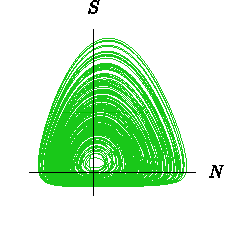
\includegraphics[width=0.25\textwidth]{figures/attractor.pdf}
    \hspace{5 mm}
    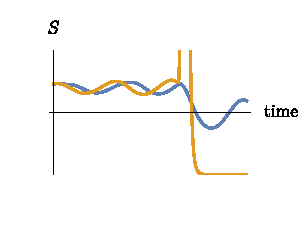
\includegraphics[width=0.35\textwidth]{figures/ics.pdf}
    %\caption{}
    %\label{fig:}
\end{figure}

\vspace{-5mm}
\begin{minipage}{0.35\textwidth}
      Possible applications:
\end{minipage}
\hfill
\begin{minipage}{0.63\textwidth}
    \begin{itemize}
        \iitem{random numbers generation;}
        \iitem{signal encryption.}
    \end{itemize}
\end{minipage}


